\documentclass[12pt,a4paper]{article}
\usepackage[T2A]{fontenc}      % кодировка
\usepackage[utf8]{inputenc}    % кодировка
\usepackage[english,russian]{babel}
\usepackage{amsmath,amssymb}   % математические пакеты
\usepackage{graphicx}          % для вставки рисунков
\usepackage{geometry}          % для задания полей страницы
\geometry{left=2cm,right=2cm,top=2cm,bottom=2cm}

\begin{document}

\begin{titlepage}
    \thispagestyle{empty}  % убираем номера страниц на титульном листе
    \begin{center}
        \large
        Федеральное государственное автономное образовательное учреждение\\
        высшего образования\\
        <<Санкт-Петербургский государственный электротехнический университет <<ЛЭТИ>>\\
        им. В.И. Ульянова (Ленина)>>\\[2em]
        
        \textbf{Кафедра физики}\\[4em]
        
        \textbf{\Large ОТЧЁТ}\\
        по лабораторной работе №\,19\\[1em]
        \textbf{\large «Исследование эффекта Холла в полупроводнике»}\\[4em]
        
        \begin{tabular}{rl}
            Выполнил: & Студент группы 4395 \\
                       & Николаев Всеволод Юрьевич \\[0.5em]
            Преподаватель: & Малышев Михаил Николаевич \\
        \end{tabular}\\[6em]
        
        \vfill
        Санкт-Петербург, 2025
    \end{center}
\end{titlepage}

\tableofcontents
\clearpage

\section{Введение}

Цель данной лабораторной работы --- исследовать влияние магнитного поля на движущиеся носители заряда в полупроводнике (с электронным типом проводимости) и определить ключевые параметры материала:
\begin{itemize}
    \item постоянную Холла $R$,
    \item концентрацию носителей заряда $n$,
    \item подвижность носителей $\mu$.
\end{itemize}
Явление Холла позволяет не только выявлять природу носителей заряда (электронная или дырочная проводимость), но и оценивать численные значения упомянутых характеристик, что имеет важное практическое значение в полупроводниковой электронике.

\section{Теоретические сведения}

\subsection{Эффект Холла}

\textbf{Эффект Холла} заключается в появлении поперечного электрического поля в проводящем образце, по которому протекает ток, при помещении образца в магнитное поле, перпендикулярное направлению тока.

Пусть в тонкой пластинке полупроводника, имеющей толщину $d$, протекает ток $I$. Если магнитное поле $\vec{B}$ направлено перпендикулярно току, то на движущиеся заряженные частицы (заряд $e$, скорость $\vec{v}$) действует сила Лоренца:
\[
    \vec{F} = e \left[\vec{v} \times \vec{B}\right].
\]
Она отбрасывает носители заряда к одному из краёв пластинки, в результате чего между этим краем и противоположным возникает разность потенциалов, называемая \textbf{напряжением Холла} $U_x$. Сформировавшееся поперечное электрическое поле $E_x$ уравновешивает силу Лоренца, и в установившемся режиме имеем:
\[
    e\,v\,B = e\,E_x.
\]
Если ширина пластинки равна $b$, то:
\[
    U_x = E_x \cdot b.
\]
С другой стороны, плотность тока через образец:
\[
    j = \frac{I}{b\,d} = n\,e\,v,
\]
где $n$ --- концентрация носителей заряда, $e$ --- заряд электрона, $v$ --- средняя скорость направленного движения. Из этих соотношений следует, что:
\[
    U_x = R \frac{I\,B}{d},
\]
где
\[
    R = \frac{1}{n\,e} 
\]
называется \textbf{постоянной Холла}. Определив $R$ экспериментально, можно найти концентрацию $n = 1/(R\,e)$. Знак $U_x$ даёт информацию о типе проводимости: при электронном типе $U_x$ положительно (для выбранного направления тока), при дырочном --- отрицательно (или наоборот, в зависимости от стандарта подключения).

\subsection{Подвижность носителей заряда}

\textbf{Подвижность} $\mu$ описывает, с какой скоростью перемещаются носители заряда под действием электрического поля. Для полупроводника с концентрацией $n$ электронов формула для удельной проводимости $\sigma$:
\[
    \sigma = n\,e\,\mu.
\]
Поскольку 
\[
    R = \frac{1}{n\,e},
\]
то:
\[
    \mu = \sigma \, R.
\]
Значение $\sigma$ может быть определено из независимых измерений сопротивления образца с учётом его геометрии или известно по данным о материале.

\subsection{Магнитное поле электромагнита}

В работе используется электромагнит, состоящий из двух соосных катушек на магнитопроводе. При заданных токах $I_2$ в катушках (в амперах) магнитная индукция $B$ в рабочей области (где размещён датчик Холла) аппроксимируется формулой:
\[
    B = B_{\text{н}} + a\,I_2,
\]
где:
\begin{itemize}
    \item $B_{\text{н}}$ --- начальная (остаточная) индукция сердечника,
    \item $a$ --- коэффициент пропорциональности,
    \item $I_2$ --- сила тока через обмотки.
\end{itemize}

\section{Описание экспериментальной установки}

\subsection{Основные элементы стенда}

\begin{itemize}
    \item \textbf{Датчик Холла (ДХ)}: полупроводниковая плёнка (или пластинка), напылённая на диэлектрическую подложку, с четырьмя выводами. Два из них --- для пропускания тока $I_1$, ещё два --- для съёма напряжения Холла $U_x$.
    \item \textbf{Электромагнит (ЭМ)}: создаёт магнитное поле, перпендикулярное плоскости ДХ. Ток в катушках задаётся источником питания $E_2$ и потенциометром $R_2$.
    \item \textbf{Источники питания}:
          \begin{itemize}
              \item $E_1$ --- для подачи тока $I_1$ через ДХ,
              \item $E_2$ --- для питания катушек электромагнита (обеспечивает $I_2$).
          \end{itemize}
    \item \textbf{Регулируемые резисторы (потенциометры)}:
          \begin{itemize}
              \item $R_1$ (<<Ток ДХ>>) --- регулирует $I_1$,
              \item $R_2$ (<<Ток ЭМ>>) --- регулирует $I_2$.
          \end{itemize}
    \item \textbf{Измерительные приборы}:
          \begin{itemize}
              \item Миллиамперметр (mA) --- показывает $I_1$ (в мА),
              \item Вольтметр $V2$ --- измеряет падение напряжения на резисторе $R=1\,\Omega$, так что его показания равны току $I_2$ (в А),
              \item \textbf{Операционный усилитель} (ОУ) с коэффициентом усиления $k$ --- усиливает сигнал Холла $U_x$,
              \item Вольтметр $V1$ --- измеряет выход ОУ ($U_1$), откуда $U_x = U_1 / k$.
          \end{itemize}
\end{itemize}

\subsection{Схема подключения}

На рисунке условно показан общий вид схемы:

\begin{figure}[h!]
    \centering
    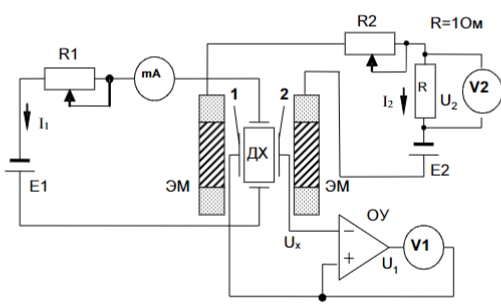
\includegraphics[width=0.55\textwidth]{hall_scheme.png}
    \caption{Принципиальная схема установки для исследования эффекта Холла.}
    \label{fig:scheme}
\end{figure}

Ключевые элементы схемы (ДХ, ЭМ, R=1~Ом, OУ, вольтметры, миллиамперметр, потенциометры) связаны так, чтобы:
\begin{itemize}
    \item задавать ток $I_1$ в датчике Холла,
    \item контролировать магнитное поле (ток $I_2$ в электромагните),
    \item усиливать малое напряжение Холла,
    \item регистрировать его удобным для измерения вольтметром.
\end{itemize}

\section{Методика выполнения работы}

\subsection{Подготовка к измерениям}

\begin{enumerate}
    \item Установить пределы измерений на приборах:
          \begin{itemize}
              \item миллиамперметр (mA): <<200\,mA>> или соответствующий близкий диапазон,
              \item вольтметр $V2$: <<20\,VDC>> (при $R=1\,\Omega$ даёт измерения тока до 20\,A, но в практике обычно $\leq 1$\,A),
              \item вольтметр $V1$: <<20\,VDC>> для контроля выходного напряжения ОУ.
          \end{itemize}
    \item Вывести потенциометры $R_1$ (<<Ток ДХ>>) и $R_2$ (<<Ток ЭМ>>) в крайние левые положения (минимум тока).
    \item Включить источники питания $E_1$ и $E_2$.
\end{enumerate}

\subsection{Съём экспериментальных данных}

\begin{enumerate}
    \item \textbf{Задание тока $I_1$.} Потенциометром $R_1$ установить нужную величину тока в датчике Холла (например, 2\,mA). Зафиксировать по миллиамперметру (mA). 
    \item \textbf{Изменение тока в электромагните $I_2$.} Потенциометром $R_2$ плавно увеличить $I_2$ от минимума (0--0.1\,A) до максимума (около 1\,A). На каждом шаге зафиксировать значение $I_2$ (по $V2$) и выходное напряжение $U_1$ (по $V1$).
    \item \textbf{Повтор} для нескольких (5 и более) значений $I_1$ (2\,mA, 4\,mA, 6\,mA и т.\,д.), повторяя набор точек по $I_2$.
    \item После съёма всех точек уменьшить токи $I_2$ и $I_1$, выключить питание.
\end{enumerate}

\end{document}
